\subsection{การดิสครีไทซ์เซชันแบบไฟไนต์ดิฟเฟอเรนจ์}

\hspace{1cm}ไฟไนต์ดิฟเฟอร์เรนจ์ (Finite Difference) คือวิธีการสำหรับการประมาณค่าอนุพันธ์เมื่อใช้วิธีเชิงตัวเลข ซึ่งในโครงงานวิจัยชิ้นนี้จะมีตัวดำเนินการที่เกี่ยวข้องกับอนุพันธ์ด้วยกัน 3 ตัวได้แก่ แกรเดียน ไดเวอร์เจน และ ลาปาเซียนซึ่งสามารถทำการหาได้ดังนี้

\subsubsection{การหาอนุพันธ์}

\hspace{1cm}ทั้ง แกรเดียน ไดเวอร์เจน และ ลาปาเซียน ล้วนมีพื้นฐานมาจากการหาค่าอนุพันธ์ในโครงงานวิจัยนี้จะใช้วิธีการฟอร์เวิร์ดดิฟเฟอร์เรนจ์ (Forward Difference) และใช้เงื่อนไขค่าขอบแบบนิวแมน (neumann boundary condition)

\noindent\hspace{1cm}นั่นคือการหาอนุพันน์ของค่าความเข้มที่พิกัดทางกายภาพเป็น $(i,j)$
\begin{align*}
	\frac{d}{dx} u_{i,j} = \frac{u_{i,j+1} - u_{i,j}}{h}
\end{align*}

เมื่อระบบกริดที่ใช้มีความห่างเพียงหนึ่งหน่วย จึงได้ว่า $h=1$ ทั้งนี้ระยะห่าง $h$ อาจเปลี่ยนไปตามชั้นของพีระมิดรูปภาพ

\begin{figure}[H]
    \centering
    \begin{subfigure}{0.95\linewidth}
        \centering
        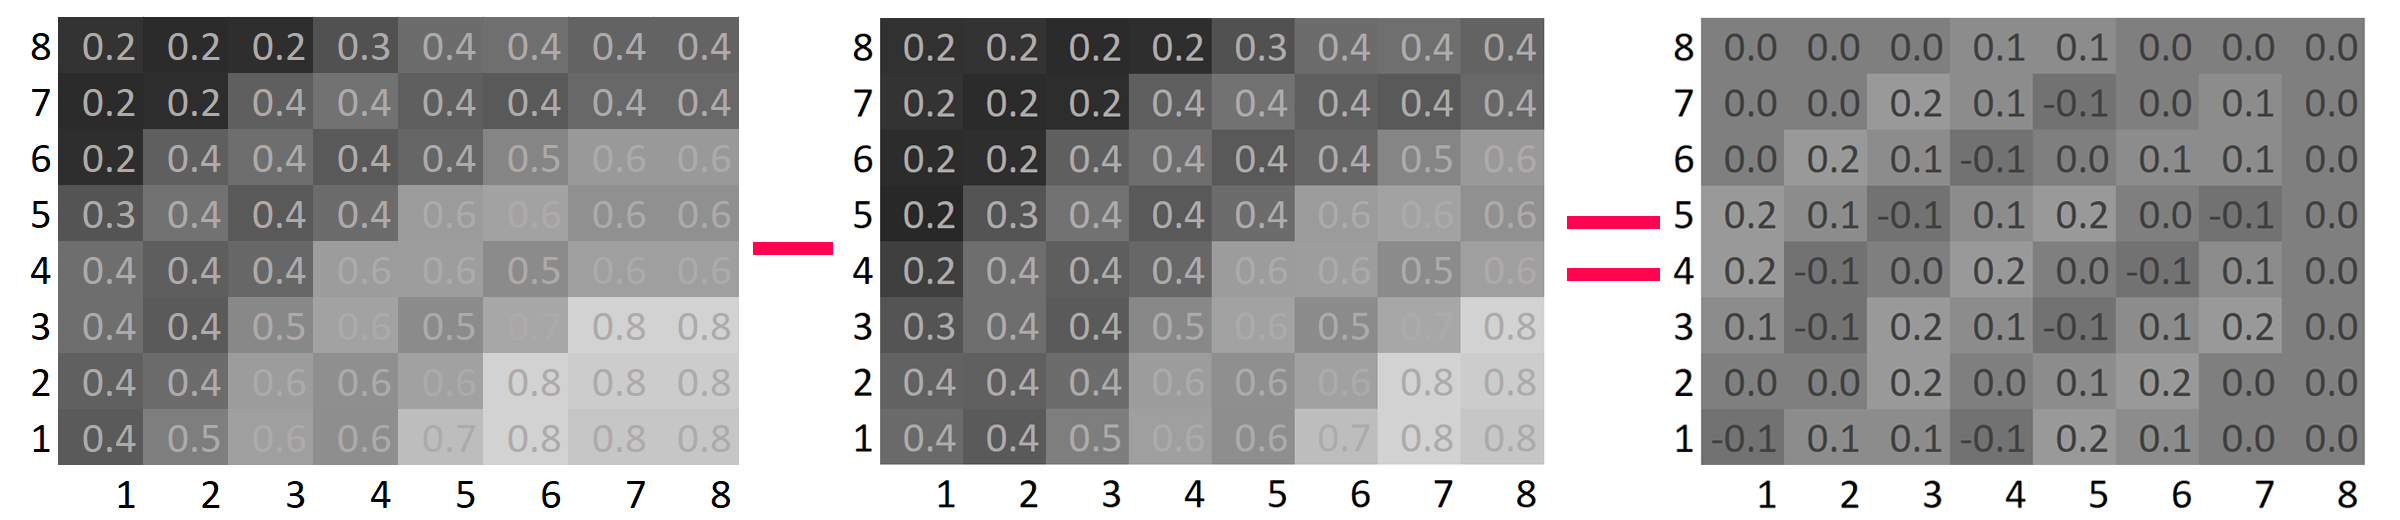
\includegraphics[width=0.9\linewidth]{image/finite_difference/x_derivertive.png}
    \end{subfigure}
    \caption{ตัวอย่างการหาอนุพันธ์บนภาพเฉดเทา}
    \label{figure:x-derivertive}
\end{figure}

\hspace{1cm} จากภาพ \ref{figure:grayscale-explain} เมื่อต้องการหาอนุพันธ์เทียบแกน x จะทำตามภาพที่ \ref{figure:x-derivertive}โดยทำการสร้างภาพซึ่งทำการตัดขอบทางซ้ายออกหนึ่งคอลัมม์และเพิ่มขอบทางขวาหนึ่งคอลัมม์โดยใช้เงื่อนไขค่าขอบแบบนิวแมน จากนั้นภาพที่สร้างขึ้นไปลบกับภาพเดิมจะได้อนุพันธ์ของภาพนั้นดังที่ปรากฏทางขวา ทั้งนี้หาก $ h \neq 1 $ สามารถทำการหารภาพผลลัพธ์ด้วยค่า $h$ ได้เพื่อให้ได้ค่าที่ต้องการ

\subsubsection{การหาแกรเดียน}
\noindent\hspace{1cm}สำหรับการหาแกรเดียน (Gradient) จะใช้การหาอนุพันธ์โดยวิธีฟอร์เวิร์ดดิฟเฟอร์เรนจ์ดังที่กล่าวไปในหัวข้อก่อนหน้า ั้งในแนวแกน x และแนวแกน y คำตอบที่ได้จะเป็นเวคเตอร์ของอนุพันธ์แนวแกน x และอนุพันธ์แนวแกน y  ได้เวคเตอร์ดังนี้ 

\begin{align*}
	\nabla \vec{v_{u_i}} = (\frac{d}{dx} u_{i,j},\frac{d}{dy} u_{i,j})^{\top}	
\end{align*}

\subsubsection{การหาไดเวอร์เจน}
\noindent\hspace{1cm}สำหรับไดเวอร์เจน (Divergence) จะเป็นการหาผลรวมของอนุพันธ์ในแต่ละแกนของเวคเตอร์ด้วยวิธีฟอร์เวิร์ดดิฟเฟอร์เรนจ์ นั่นคือ 

\begin{align*} 
	\nabla \cdot (\vec{v_{i,j}}) = \frac{\partial d}{\partial x}\vec{v_{i,j}}_x + \frac{\partial d}{\partial y}\vec{v_{i,j}}_y
\end{align*}

\subsubsection{การหาลาปาเชียน}
\noindent\hspace{1cm}สำหรับลาปาเซียน (Lapacian) นั่นคือการทำหาไดเวอร์เจรบนเวคเตอร์ที่หาแกรเดียนแล้ว แต่ทั้งนี้สามารถหาลาปาเชียนได้จาก

\begin{align*}
	\triangle u_{i,j} = u_{i-1,j} + u_{i+1,j} + u_{i,j-1} + u_{i,j+1} - 4 u_{i,j} 
\end{align*}